\documentclass{article}
\title{CS310 Final Report \\ The Use of Gamification and Analytics in Higher Education}
\author{William Seymour, Third Year Computer Science \\ Supervisor: Mike Joy}
\date{\today}
\linespread{1.3}

\usepackage{cite}
\usepackage{graphicx}
\usepackage{url}

\begin{document}
\maketitle
\clearpage
\tableofcontents

\section{Abstract}
Gamification and analytics are becoming increasingly popular in many facets of everyday life. They are making a big impact in primary and secondary education, driven by the increased use of internet enabled devices in the classroom. This project looks at how this can be translated to higher education, and what role the traditional gamification personality types might have in this field.

\section{Key words}
Gamification, Classroom analytics, Higher education, Flipped classroom

\section{Introduction}
It seems an obvious fact of life that work is dull, and play is fun. Many attempts have been made to change this, but they have largely been met with little success. Over the past few years, gamification has been slowly blurring the line between what is considered to be `work', by slowly moving it towards practises and behaviours that would normally be associated with play. Coupled with the advanced user tracking and analytics offered by modern technology, it has begun to dominate the ways in which we interact electronically, with services like Facebook and Foursquare being prime examples. The benefit of integrating these techniques into primary and secondary education was clear from the beginning, but there has been less enthusiasm for its use in higher education. This report seeks to assess the usefulness of the aforementioned techniques in the higher education sector, and what form they might take when used to greatest effect. It will also explore the application of the traditional Bartle personality types used in gamification, with particular interest in how useful (or not) they might be in directing teaching and learning.

\section{Background}
Gamification is a fairly young field of study, the term having only really gained popularity in late 2010, as shown in figure \ref{usagegraph}. Its recent discovery has meant that far less has been done to incorporate developments on gamification into the current education system. While outside the scope of the project, one question that remains to be answered is how the engagement increases from gamification hold up when its use becomes widespread: is it only an increase relative to content that is not gamified, or can it offer an absolute increase in engagement?

The success of gamification in driving engagement has underlying roots in psychology, with gameified experiences being able to satisfy more psychological needs than what might normally be considered `work'. For example, the feedback mechanisms which typify these experiences, such as progress bars, badges and the awarding of in-game points, help fulfil the need for competence experienced by all human beings \cite{przybylski2010motivational}. Players are compelled to complete game actions in order to feel capable, and challenges often use time investment as the principal measure of worth. Traditional games tend to confer rewards and status based on skill, which alienates a large proportion of the player base who fall outside the top performers. In this way all players feel as if they can succeed if they play the game for long enough, or regularly enough.

\begin{figure}
	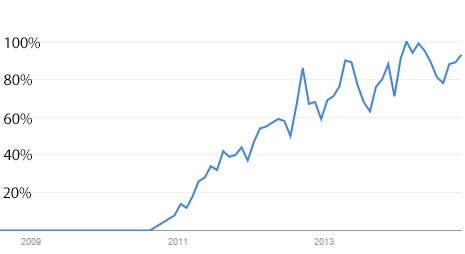
\includegraphics{../img/usage-graph.png}
	\caption{Usage of the term `gamification' by month as a proportion of the total number of google searches for gamification, from 2009 to the present day \cite{usage}}
	\label{usagegraph}
\end{figure}

\section{Definitions}
It is important to define some of the key terms that will be used in this report. Terms like gamification and analytics are often bandied around by lots of different parties who all mean similar but subtly different things. Indeed, the way in which these terms have been used thus far have been somewhat unclear. For the remainder of the document, the undermentioned should be referred to as a definitive explanation of what is meant by the following technical terms:

\subsection{Gamification}
A commonly accepted definition of gamification is that it is the use of game design elements in non-game contexts \cite{deterding2011game}. This is a good in that it makes clear the distinction between games and gamified activities, but what exactly counts as either can often be left unclear. This is difficult as it is near impossible to pin down where one stops and the other begins. This is likely to increase as game elements are further incorporated into everyday activities, and seems to suggest that rigorously defining what is and is not a game is of less value than originally anticipated. Here, a game [man, play and games put on hold].

Game elements also need to be outlined in a little more depth. For the purposes of this project, it will be taken to mean those elements of game systems which compel users to play because they are engaging or fun. Alternatively put, the focus is on the mechanics that make games interesting and keep users coming back as opposed to graphical techniques or the platforms they reside on. This  Further definition, as before, carries the risk of splitting hairs, and does not add much to the discussion.

\subsection{Analytics}

\section{Legal, Social, Ethical and Professional Issues}

\section{Conclusion and Further Work}

\section{Background Texts}

\bibliography{references}
\bibliographystyle{plain}
\end{document}